\documentclass[aspectratio=169,notes]{beamer}
\usepackage{lmodern}
\usepackage{adjustbox}
\usepackage[T1]{fontenc}
\usepackage{textcomp}
\usepackage{animate}
\usepackage{underscore}
\usepackage{pdfpc-commands}
\usepackage{xmpmulti}
\usepackage{multimedia}
\usepackage{epstopdf}
\usepackage{bbding}

\definecolor{Title}{rgb}{0.94,0.52,0.08}
\setbeamercolor{frametitle}{bg=Title,fg=black}

% footnote without number
\makeatletter
\def\blfootnote{\xdef\@thefnmark{}\@footnotetext}
\makeatother

\usepackage{hyperref}
\usepackage{scalerel}
\def\thumbup{\scalerel*{
\includegraphics{thumbup.png}}{O}}
\usepackage{listings}
\lstdefinelanguage{D}
{
  % list of keywords
  morekeywords={ abstract, alias, align, asm, assert, auto, body, bool, break,
	byte, case, cast, catch, cdouble, cent, cfloat, char, class, const,
	continue, default, double, else, enum, export, extern, false, final, finally,
	float, for, foreach, foreach_reverse, function, goto, idouble, if, ifloat,
	immutable, import, in, inout, int, interface, invariant, ireal, is, lazy,
	long, mixin, module, new, nothrow, null, out, override, package, pragma,
	private, protected, public, pure, real, ref, return, scope, shared, short,
	static, string, struct, super, switch, synchronized, template, this, throw,
	true, try, typeid, typeof, ubyte, ucent, uint, ulong, union,
	unittest, delegate, @safe
	ushort, version, void, wchar, while, with, __FILE__, __FILE_FULL_PATH__,
	__MODULE__, __LINE__, __FUNCTION__, __PRETTY_FUNCTION__, __gshared,
	__traits, __vector, __parameters
  },
  sensitive=false, % keywords are not case-sensitive
  morecomment=[l]{//}, % l is for line comment
  morecomment=[s]{/*}{*/}, % s is for start and end delimiter
  morecomment=[s]{/+}{+/}, % s is for start and end delimiter
  morestring=[b]" % defines that strings are enclosed in double quotes
}
\usepackage{color}
\definecolor{eclipseBlue}{RGB}{42,0.0,255}
\definecolor{eclipseGreen}{RGB}{63,127,95}
\definecolor{eclipsePurple}{RGB}{127,0,85}

% Set Language
\lstset{
  language={D},
  basicstyle=\small\ttfamily, % Global Code Style
  captionpos=b, % Position of the Caption (t for top, b for bottom)
  extendedchars=true, % Allows 256 instead of 128 ASCII characters
  tabsize=2, % number of spaces indented when discovering a tab 
  columns=fixed, % make all characters equal width
  keepspaces=true, % does not ignore spaces to fit width, convert tabs to spaces
  showstringspaces=false, % lets spaces in strings appear as real spaces
  breaklines=true, % wrap lines if they don't fit
  numbers=left, % show line numbers at the left
  numberstyle=\tiny\ttfamily, % style of the line numbers
  commentstyle=\color{eclipseGreen}, % style of comments
  keywordstyle=\color{eclipsePurple}, % style of keywords
  stringstyle=\color{eclipseBlue}, % style of strings
}
\definecolor{lightgray}{rgb}{.9,.9,.9}
\definecolor{darkgray}{rgb}{.4,.4,.4}
\definecolor{purple}{rgb}{0.65, 0.12, 0.82}
\lstdefinelanguage{TypeScript}{
	keywords={break, case, catch, continue, debugger, default, delete, do, else,
		false, from, finally, for, function, if, in, instanceof, new, null, return, switch,
		this, throw, true, try, typeof, var, void, while, with, interface,
		class, export, boolean, throw, implements, import, this, const, let,
		of, =>},
	morecomment=[l]{//},
	morecomment=[s]{/*}{*/},
	morestring=[b]',
	morestring=[b]",
	ndkeywords={},
	keywordstyle=\color{blue}\bfseries,
	ndkeywordstyle=\color{darkgray}\bfseries,
	identifierstyle=\color{black},
	commentstyle=\color{purple}\ttfamily,
	stringstyle=\color{red}\ttfamily,
	sensitive=true
}

\colorlet{punct}{red!60!black}
\definecolor{background}{HTML}{EEEEEE}
\definecolor{delim}{RGB}{20,105,176}
\colorlet{numb}{magenta!60!black}

\lstdefinelanguage{GraphQL}{
    basicstyle=\normalfont\ttfamily,
    numbers=left,
    stepnumber=1,
    showstringspaces=false,
    breaklines=true,
	keywords={type, schema, mutation, subscription, __type, __schema, kind,
		on, fragment, query},
    literate=
     *{0}{{{\color{numb}0}}}{1}
      {1}{{{\color{numb}1}}}{1}
      {2}{{{\color{numb}2}}}{1}
      {3}{{{\color{numb}3}}}{1}
      {4}{{{\color{numb}4}}}{1}
      {5}{{{\color{numb}5}}}{1}
      {6}{{{\color{numb}6}}}{1}
      {7}{{{\color{numb}7}}}{1}
      {8}{{{\color{numb}8}}}{1}
      {9}{{{\color{numb}9}}}{1}
      {:}{{{\color{punct}{:}}}}{1}
      {,}{{{\color{punct}{,}}}}{1}
      {\{}{{{\color{delim}{\{}}}}{1}
      {\}}{{{\color{delim}{\}}}}}{1}
      {[}{{{\color{delim}{[}}}}{1}
      {]}{{{\color{delim}{]}}}}{1},
}

\lstdefinelanguage{json}{
    basicstyle=\normalfont\ttfamily,
    numbers=left,
    stepnumber=1,
    showstringspaces=false,
    breaklines=true,
    literate=
     *{0}{{{\color{numb}0}}}{1}
      {1}{{{\color{numb}1}}}{1}
      {2}{{{\color{numb}2}}}{1}
      {3}{{{\color{numb}3}}}{1}
      {4}{{{\color{numb}4}}}{1}
      {5}{{{\color{numb}5}}}{1}
      {6}{{{\color{numb}6}}}{1}
      {7}{{{\color{numb}7}}}{1}
      {8}{{{\color{numb}8}}}{1}
      {9}{{{\color{numb}9}}}{1}
      {:}{{{\color{punct}{:}}}}{1}
      {,}{{{\color{punct}{,}}}}{1}
      {\{}{{{\color{delim}{\{}}}}{1}
      {\}}{{{\color{delim}{\}}}}}{1}
      {[}{{{\color{delim}{[}}}}{1}
      {]}{{{\color{delim}{]}}}}{1},
}
\usepackage{tikz}
\usetikzlibrary{shadows,calc}
\usepackage{xkeyval}
\usepackage{todonotes}
\presetkeys{todonotes}{inline}{}
\defbeamertemplate{description item}{align left}{\insertdescriptionitem\hfill}
\usetheme{metropolis}					 % Use metropolis theme
\usepackage[
    backend=biber,
	sorting=none,
    url=true 
]{biblatex}
\addbibresource{biblio.bib}
\setbeamertemplate{bibliography item}{\insertbiblabel}

\title{All Spreadsheets must Die}
\date{\today}
\author{Robert Schadek}
\begin{document}
	\maketitle

	\section{Getting started}
	\begin{frame}[fragile]{A random list of languages we love to hate}
		\begin{tikzpicture}[remember picture,overlay]
  			\node[anchor=south west,inner sep=0pt, rotate=15] at ($(current page.south west)+(2cm,3cm)$) {
				
\includegraphics[width=30mm]{cpplogo.eps}
			};
  			\node[anchor=south west,inner sep=0pt, rotate=-15] at ($(current page.south west)+(5cm,4cm)$) {
				
\includegraphics[width=30mm]{rustlogo.eps}
			};
  			\node[anchor=south west,inner sep=0pt, rotate=2] at ($(current page.south west)+(8cm,0.5cm)$) {
				
\includegraphics[width=30mm]{golang.png}
			};
  			\node[anchor=south west,inner sep=0pt, rotate=10] at ($(current page.south west)+(9cm,4cm)$) {
				
\includegraphics[width=30mm]{tslogo.png}
			};
  			\node[anchor=south west,inner sep=0pt, rotate=-10] at ($(current page.south west)+(5cm,0.5cm)$) {
				
\includegraphics[width=30mm]{clogo.png}
			};
  			\node[anchor=south west,inner sep=0pt, rotate=-20] at ($(current page.south west)+(10cm,0.5cm)$) {
				
\includegraphics[width=30mm]{jslogo.png}
			};
  			\node[anchor=south west,inner sep=0pt, rotate=-20] at ($(current page.south west)+(11.5cm,4.0cm)$) {
				
\includegraphics[width=30mm]{javalogo.png}
			};
  			\node[anchor=south west,inner sep=0pt, rotate=0] at ($(current page.south west)+(13.0cm,1.0cm)$) {
				
\includegraphics[width=30mm]{csharp.png}
			};
  			\node[anchor=south west,inner sep=0pt, rotate=20] at ($(current page.south west)+(1cm,0cm)$) {
				
\includegraphics[width=30mm]{dlogo.png}
			};
  			\node[anchor=south west,inner sep=0pt, rotate=20] at ($(current page.south west)+(4cm,1.5cm)$) {
				
\includegraphics[width=30mm]{pythonlogo.png}
			};
		\end{tikzpicture}
	\end{frame}

	\note[itemize]{
		\item There are all these languages we like to hate.
		\item Many of them are good, many are more popular.
		\item Many might even be better than D in some regards.
		\item But we are missing something
	}

	\begin{frame}{Hating by numbers}
		\begin{description}
			\item[C++] $4.4 Million$ (2015)
			\item[C] $1.9 Million$ (2015)
			\item[Java] $9 Million$ (2009)	
			\item[JS] $10 Million$ (2018)
		\end{description}
		\blfootnote{\cite{cdevs,Develope3:online}}
	\end{frame}

	\note[itemize]{
		\item Many of the languages are used by more people than D is.
		\item Programms written in C run the world (linux).
		\item JS is eating everything.
	}
	
	\begin{frame}{\mbox{}}
		\begin{center}
		\huge
		These are all small fish\\[15mm]
		\pause
		\textbf{\Huge{Excel}}\\[15mm]
		$\approx{} 750$ Million (2016)
		\only<2->{\footnote{\cite{Build20153:online,Sevenrea2:online}}}
		\end{center}
	\end{frame}

	\begin{frame}[fragile]{\mbox{}}
		\begin{tikzpicture}[remember picture,overlay]
  			\node[anchor=south west,inner sep=0pt, rotate=0] at ($(current page.south west)+(4cm,0cm)$) {
				
\includegraphics[width=0.6\textwidth]{skeptical1.png}
			};
		\end{tikzpicture}
	\end{frame}

	\begin{frame}[fragile]{\mbox{}}
		\begin{tikzpicture}[remember picture,overlay]
  			\node[anchor=south west,inner sep=0pt, rotate=0] at ($(current page.south west)+(4cm,0cm)$) {
				
\includegraphics[width=0.6\textwidth]{skeptical2.png}
			};
		\end{tikzpicture}
	\end{frame}

	\begin{frame}[fragile]{Oh, but it is \hfill{} \cite{GOTO201638:online}}
		\begin{center}
		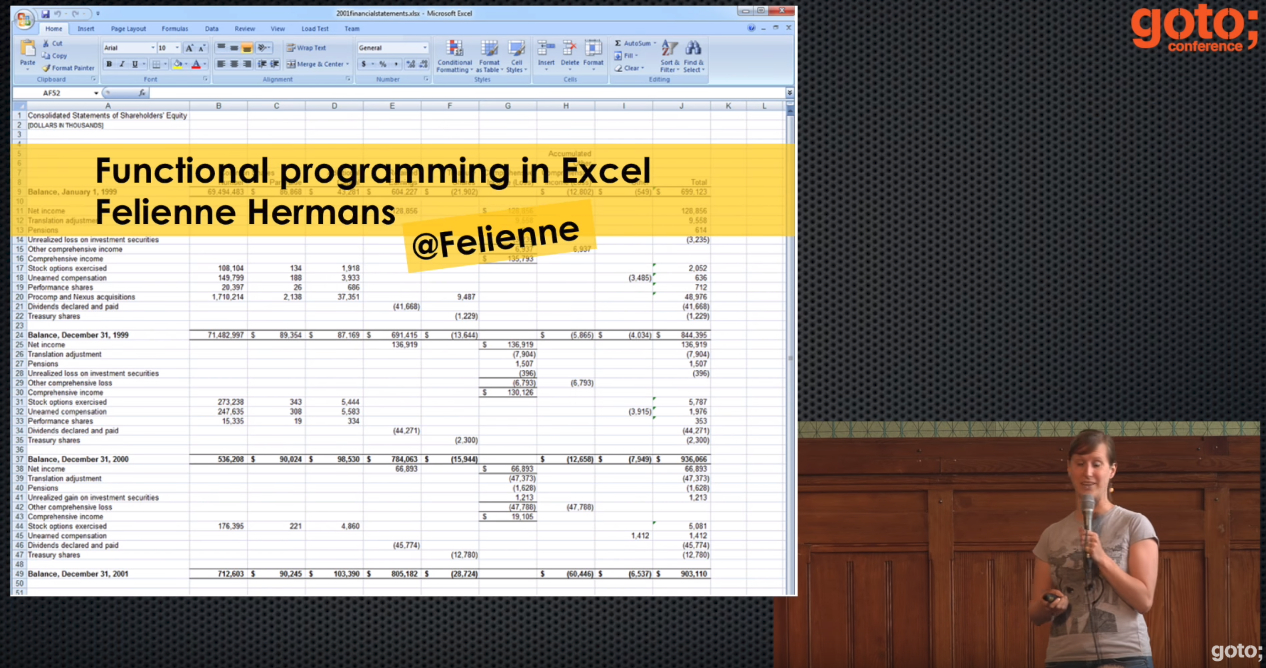
\includegraphics[width=1.0\textwidth]{functionalexcel.jpg}
		\end{center}
	\end{frame}

	\section{A little bit of Spreadsheet bashing}
	\begin{frame}[fragile]{Seeing the code is difficult}
		\begin{center}
		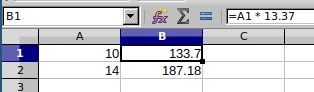
\includegraphics[width=1.0\textwidth]{excelseeingcode.jpg}
		\end{center}
	\end{frame}

	\begin{frame}[fragile]{Dynamic Types}
		\begin{center}
		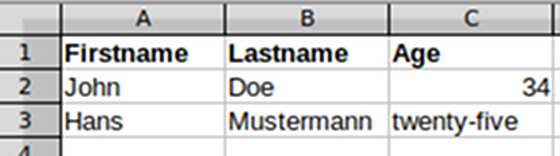
\includegraphics[width=1.0\textwidth]{exceldynamic.jpg}
		\end{center}
	\end{frame}

	\begin{frame}[fragile]{Dynamic Types}
		\begin{center}
		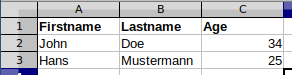
\includegraphics[width=1.0\textwidth]{exceldynamic2.jpg}
		\end{center}
	\end{frame}

	\begin{frame}[fragile]{Dynamic Types}
		\begin{center}
		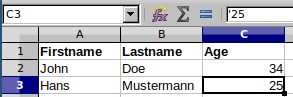
\includegraphics[width=1.0\textwidth]{exceldynamic3.jpg}
		\end{center}
	\end{frame}

	\begin{frame}[fragile]
		\begin{center}
		
\includegraphics[width=0.8\textwidth]{picard.png}
		\end{center}
	\end{frame}

	\begin{frame}[fragile]{git blame}
		\begin{center}
			\Large
			git blame\\[2cm]
			\pause
			\Huge
			lets not go there
			\only<2->{\blfootnote{we will just become sad}}
		\end{center}
	\end{frame}

	\begin{frame}[fragile]{Code refactoring}
		\Large
		\begin{itemize}
			\item \lstinline@=SUM(1,2)@ \pause
			\item equal, identifier, lparen, int(1), comma, int(2), rparen\\[5mm] \pause
			\item set excel locale to de\_DE
			\item \lstinline@=SUM(1,2)@ \pause
			\item equal, identifier, lparen, float(1.2), rparen
		\end{itemize}
	\end{frame}

	\note[itemize]{
		\item Who cares about rvalues or named arguments.
		\item I want this in D.
	}

	\begin{frame}[fragile]{Bits and Pieces}
		\Large
		\begin{itemize}
			\item Knowledge silos
			\item Slow	
			\item No separation between data and code
			\item Access management $\dots$ \pause anybody?
		\end{itemize}
	\end{frame}

	\begin{frame}[fragile]{(Typical) Spreadsheet Lifecycle}
		\Large
		\begin{enumerate}
			\item Create private shopping spreadsheet
			\item Show spreadsheet to college 
			\item Use spreadsheet for all company purchases
			\item Put web frontend on spreadsheet backend
			\item Pivot company to become commerce company
		\end{enumerate}	
		\pause
		\begin{tikzpicture}[remember picture,overlay]
		    \node[drop shadow,xshift=75mm,yshift=-38mm,rotate=-15,anchor=north west] 
				at (current page.north west){
\includegraphics[width=50mm]{snafu.jpg}};
			\pause
		    \node[drop shadow,xshift=35mm,yshift=-38mm,rotate=15,anchor=north west] 
				at (current page.north west){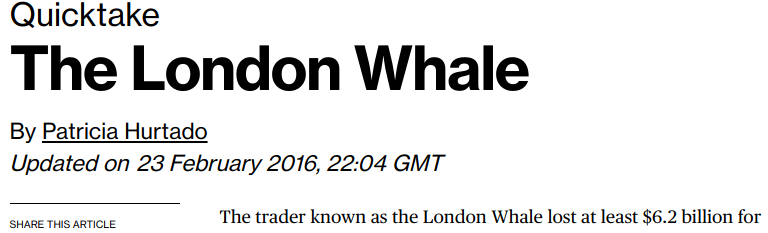
\includegraphics[width=50mm]{snafu2.jpg}};
			\pause
		    \node[drop shadow,xshift=75mm,yshift=-38mm,rotate=-35,anchor=north west] 
				at (current page.north west){
\includegraphics[width=50mm]{snafu3.jpg}};
			\pause
		    \node[drop shadow,xshift=75mm,yshift=-38mm,rotate=35,anchor=north west] 
				at (current page.north west){
\includegraphics[width=50mm]{snafu4.jpg}};
			\pause
		    \node[drop shadow,xshift=40mm,yshift=-33mm,rotate=15,anchor=north west] 
				at (current page.north west){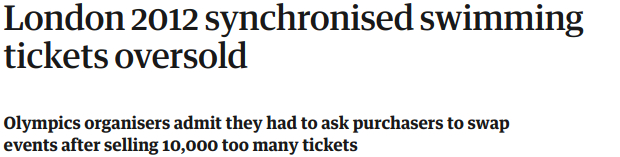
\includegraphics[width=50mm]{snafu5.jpg}};
			\pause
		    \node[drop shadow,xshift=55mm,yshift=-18mm,rotate=15,anchor=north west] 
				at (current page.north west){
\includegraphics[width=50mm]{snafu6.jpg}};
			\pause
		    \node[drop shadow,xshift=55mm,yshift=-28mm,rotate=5,anchor=north west] 
				at (current page.north west){
\includegraphics[width=50mm]{snafu7.jpg}};
			\pause
		    \node[drop shadow,xshift=35mm,yshift=-28mm,rotate=-17,anchor=north west] 
				at (current page.north west){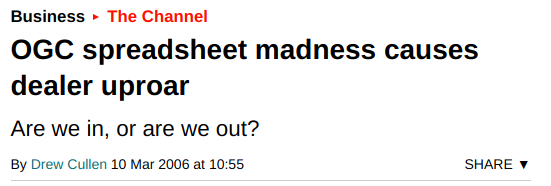
\includegraphics[width=50mm]{snafu8.jpg}};
			\pause
		    \node[drop shadow,xshift=35mm,yshift=-28mm,rotate=17,anchor=north west] 
				at (current page.north west){
\includegraphics[width=50mm]{snafu10.jpg}};
			\pause
		    \node[drop shadow,xshift=35mm,yshift=-15mm,rotate=0,anchor=north west] 
				at (current page.north west){
\includegraphics[width=70mm]{snafu9.jpg}};
		\end{tikzpicture}
	\end{frame}
	
	\begin{frame}
		\begin{center}
			\huge
			\textbf{Spreadsheets rule the world!}
		\end{center}
	\end{frame}
	
	\begin{frame}{How you should be feeling right now}
		\begin{center}
    		\inlineMovie[loop&autostart&start=0&stop=12]{kermit.mpg}{kermit-0.png}{height=0.9\textheight}
		\end{center}
	\end{frame}

	\begin{frame}{Two assumptions going forward}
		\huge
		\begin{enumerate}
			\item You believe that spreadsheets rule the world.
			\item You want D to rule the world instead.
		\end{enumerate}
	\end{frame}

	\begin{frame}{\mbox{}}
		\begin{center}
			\huge
			How are we going to win this?\\[2cm]
			\pause
			We are not!
		\end{center}
	\end{frame}

	\section{Lets draw up a battle plan}

	\begin{frame}{Lets take stock of what we have}
		\large
		\begin{itemize}
			\item Too many spreadsheets
			\item Too many tasks
			\item Too little man-power\\[1cm] \pause
			\item Millions of lines of source in different languages
			\item D
		\end{itemize}
	\end{frame}

	\begin{frame}{Possible Attack Vectors}
		\begin{center}
		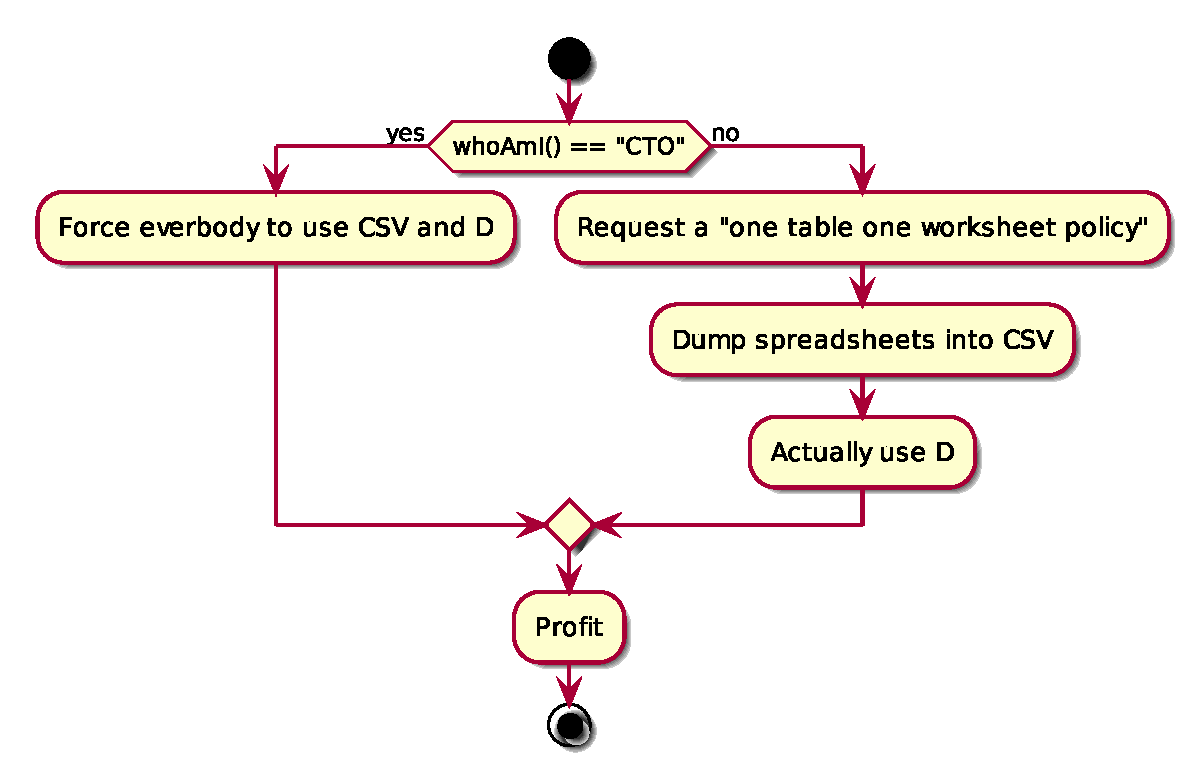
\includegraphics[width=0.8\textwidth]{attackvectors.eps}
		\end{center}
	\end{frame}

	\section{How to work with limited man-power}

	\begin{frame}{Leveraging existing libraries}
		\large
		Writing data to spreadsheets
		\pause
		\begin{itemize}
			\item Is required, people will ask for that
			\item Writing a somewhat feature complete xlsx writer is a huge task\\[1cm]
		\end{itemize}
		\begin{itemize}
			\item libxlsxwriter is a feature rich xlsx writer
			\item Wrapping it by hand, \pause no way (+78000 lines of structs, enums and functions)\\[1cm]
			\pause
			\item dpp to the rescue
			\item libxlsxwriter.d (+4000 lines)
			\item But it is still a C api
		\end{itemize}
	\end{frame}

	\begin{frame}[fragile]{dpp output}
		\begin{lstlisting}[language=D,basicstyle=\small\ttfamily]
void chart_axis_set_name(lxw_chart_axis*, const(char)*)
void chart_axis_set_name_range(lxw_chart_axis*, const(char)*, lxw_row_t, lxw_col_t)
void chart_axis_set_name_font(lxw_chart_axis*, lxw_chart_font*)
void chart_axis_set_num_font(lxw_chart_axis*, lxw_chart_font*)
void chart_axis_set_num_format(lxw_chart_axis*, const(char)*)
void chart_axis_set_line(lxw_chart_axis*, lxw_chart_line*)
void chart_axis_set_fill(lxw_chart_axis*, lxw_chart_fill*)
void chart_axis_set_pattern(lxw_chart_axis*, lxw_chart_pattern*)
\end{lstlisting}
	\end{frame}

	\begin{frame}[fragile]{Semi-automatic refactoring}
		\begin{lstlisting}[language=D]
struct ChartAxis {
	lxw_chart_axis* handle;

	void setName(string name) { 
		chart_axis_set_name(this.handle, toStringz(name)); 
	}

	void setNameRange(string name, lxw_row_t row, 
			lxw_col_t col) 
	{
		chart_axis_set_name(this.handle, toStringz(name), row, 
				col
			);
	}
	...
}
\end{lstlisting}
	\end{frame}

	\begin{frame}[fragile]{Creating fake data}
		\pause
		\large
		Problem to solve: We needed fake data with a variety of attributes.
		\begin{itemize}
			\item Name
			\item Address
			\item i18n
			\item ...
		\end{itemize}	
		\pause
		\begin{tikzpicture}[remember picture,overlay]
  			\node[anchor=south west,inner sep=0pt, rotate=0] at ($(current page.south west)+(1cm,0cm)$) {
				
\includegraphics[width=1.0\textwidth]{lovetrianglefaker.jpg}
			};
		\end{tikzpicture}
	\end{frame}

	\note[itemize]{
		\item It hurts me to say, but just look at the packages on npmjs.
	}

	\begin{frame}[fragile]{faker.js \hfill\cite{fakerjs}}
		
\includegraphics[width=0.2\textwidth]{fakerjs.png}
		\large
		\begin{itemize}
			\item $+160$ attributes
			\item $39$ languages
		\end{itemize}
	\end{frame}

	\begin{frame}[fragile]{faker.js}
		\begin{lstlisting}[language=Java,caption={locales/de/name/name.js}]
module["exports"] = [
  "#{prefix} #{first_name} #{last_name}",
  "#{first_name} #{nobility_title_prefix} #{last_name}",
  "#{first_name} #{last_name}",
  "#{first_name} #{last_name}",
  "#{first_name} #{last_name}",
  "#{first_name} #{last_name}"
];\end{lstlisting}
	\end{frame}

	\begin{frame}[fragile]{FakeD \hfill\cite{faked}}
\begin{lstlisting}[language=D,basicstyle=\scriptsize\ttfamily]
override string nameName() {
	switch(uniform(0, 6, this.rnd)) {
		case 0:
			return format!"%s %s %s"(namePrefix(), nameFirstName(), 
					nameLastName());
		case 1:
			return format!"%s %s %s"(nameFirstName(), nameNobilityTitlePrefix(), 
					nameLastName());
		case 2:
			return format!"%s %s"(nameFirstName(), nameLastName());
		case 3:
			return format!"%s %s"(nameFirstName(), nameLastName());
		case 4:
			return format!"%s %s"(nameFirstName(), nameLastName());
		case 5:
			return format!"%s %s"(nameFirstName(), nameLastName());
		default: assert(false);
	}
}
\end{lstlisting}
	\end{frame}

	\begin{frame}[fragile]{FakeD}
\begin{lstlisting}[language=D]
import faked;

auto f = new Faker(1337);
writeln(f.nameName());

// localized to german
f = new Faker_de(1338);
writeln(f.nameName());
\end{lstlisting}
	\end{frame}

	\begin{frame}[fragile]{FakeD}
		\Large
		\begin{itemize}
			\item Input:
			\begin{itemize}
				\large
				\item Parser and Generator $\approx 1500$ lines of D
				\item A day of labor
			\end{itemize}
		\pause
			\item Output:
			\begin{itemize}
				\large
				\item Output feature equivalent $\approx 70000$ lines faker.js clone
				\item Most changes in faker.js just require a rerun of the tool to update
			\end{itemize}
		\pause
			\item Bonus:
			\begin{itemize}
				\large
				\item Created two PRs to faker.js fixing wrong template expansion	
			\end{itemize}
		\end{itemize}
	\end{frame}

	\section{Taking a step back}

	\begin{frame}[fragile]{The Wanted Output: Salary Table}
		\Large
		\begin{center}
		\begin{tabular}{l | l | r | l | l}
			Firstname & Lastname & Amount & Currency & CreatedBy \\ \hline
			Hans & Meier & 73331 & USD & Ruth Ember \\
			John & Doe & 83431 & GPB & Ruth Ember \\
			Ruth & Ember & 103431 & EUR & Hans Meier \\
		\end{tabular}	
		\end{center}
	\end{frame}

	\begin{frame}[fragile]{The starting point}
\begin{columns}
\begin{column}[t]{0.35\textwidth}
\begin{lstlisting}[language=D,basicstyle=\scriptsize\ttfamily]
class Employee {
	long id;
	DateTime createdAt;

	EmployeeInfo info;
	long infoId;
}	

class EmployeeInfo {
	long id;
	string firstname;
	string lastname;

	Salary salary;
	long salaryId;
}	
\end{lstlisting}
\end{column}
\begin{column}[t]{0.35\textwidth}
\begin{lstlisting}[language=D,basicstyle=\scriptsize\ttfamily,firstnumber=17]
class Salary {
	long id;
	Employee createdBy;
	long createdById;

	CurrencyAmount amount;
	long amountId;
}

class CurrencyAmount {
	long id;
	double amount;

	Currency currency;
	long currencyId;
}
\end{lstlisting}
\end{column}
\begin{column}[t]{0.25\textwidth}
\begin{lstlisting}[language=D,basicstyle=\scriptsize\ttfamily,firstnumber=32]
class Currency {
	long id;
	string name;
}
\end{lstlisting}
\end{column}
\end{columns}
	\end{frame}

	\begin{frame}[fragile]{The vibe.d REST interface}
\begin{lstlisting}[language=D,basicstyle=\normalsize\ttfamily]
interface Backend {
	Employee[] getAllEmployees();
	Employee getEmployee(long empId);
	EmployeeInfo getEmployeeInfo(long empInfoId);
	Salary getSalary(long salaryId);
	CurrencyAmount getCurrencyAmount(long amountId);
	Currency getCurrency(long currencyId);
}
\end{lstlisting}
	\end{frame}

	\begin{frame}[fragile]{The Frontend Code: Types}
\begin{columns}
\begin{column}{0.5\textwidth}
\begin{lstlisting}[language=typescript,basicstyle=\small\ttfamily]
interface Employee {
	id: number;
	createdAt: number;

	info?: EmployeeInfo;
	infoId: number;
}	

interface EmployeeInfo {
	id: number;
	firstname: string;
	lastname: string;

	salary?: Salary;
	salaryId: number;
}	
\end{lstlisting}
\end{column}
\begin{column}{0.5\textwidth}
\begin{lstlisting}[language=TypeScript,basicstyle=\small\ttfamily,firstnumber=17]
interface Salary {
	id: number;
	createdBy?: Employee;
	createdById: number;

	amount?: CurrencyAmount;
	amountId: number;
}

interface CurrencyAmount {
	id: number;
	amount: number;

	currency?: Currency;
	currencyId: number;
}
\end{lstlisting}
\end{column}
\end{columns}
	\end{frame}

	\begin{frame}[fragile]{The Frontend Code: Backend Service}
\begin{lstlisting}[language=TypeScript,basicstyle=\small\ttfamily,tabsize=4]
import { 
	Employee, EmployeeInfo, Salary, CurrencyAmount, Currency 
} from "model";

class Backend {
	getAllEmployees() : Employee[] { ... }
	getEmployee(empId: number): Employee { ... }
	getEmployeeInfo(empInfoId: number): EmployeeInfo { ... }
	getSalary(salaryId: number): Salary { ... }
	getCurrencyAmount(amountId: number): CurrencyAmount { ... }
	getCurrency(currencyId: number): Currency { ... }
}
\end{lstlisting}
	\end{frame}

	\begin{frame}[fragile]{The Frontend Code: Calling the Backend}
\begin{lstlisting}[language=TypeScript,basicstyle=\footnotesize\ttfamily,tabsize=2]
this.backend.getAllEmployees().pipe(
	mergeMap((emps: Employee[]) => {
		const obs = [];
		for(const emp of emps) {
			obs.push(this.backend.getEmployeeInfo(emp.infoId)
				.pipe(map((empInfo: EmployeeInfo) => {
						const ne: Employee = {...emp, info : empInfo};
						return ne;
					})
				)
			);
		}
		return forkJoin(obs);
	}),
	mergeMap((emps: Employee[]) => {
		const obs = [];
		for(const emp of emps) {
			obs.push(this.backend.getSalary(emp.info.salaryId)
				.pipe(map((sal: Salary) => {
						const ne: Employee = {...emp};
						ne.info.salary = sal;
						return ne;
					})
				)
			);
		}
		return forkJoin(obs);
	}),
\end{lstlisting}
\end{frame}

	\begin{frame}[fragile]{The Communication}
		\begin{center}
			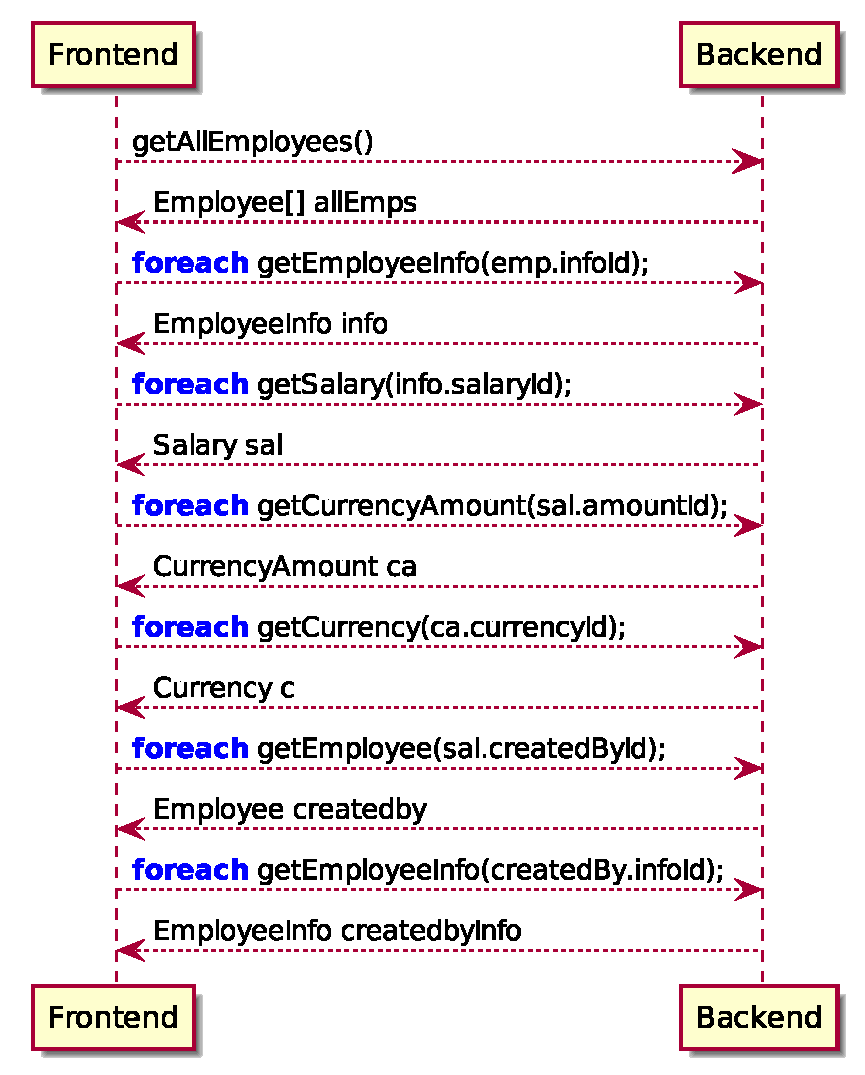
\includegraphics[height=0.9\textheight]{restbackend.eps}
		\end{center}
	\end{frame}
	
	\begin{frame}[fragile]{The Takeaways}
		\Large
		\begin{itemize}
			\item Clearly, this is unworkable
			\item Not plastic at all
			\item Just a lot of boring work
		\end{itemize}
	\end{frame}

	\begin{frame}{The real Takeway}
		\begin{center}
    		\inlineMovie[loop&autostart&start=0&stop=10]{keyboard.mpg}{keyboard-0.png}{height=0.9\textheight}
		\end{center}
	\end{frame}

	\begin{frame}{So, what do we/I want?}
		\begin{center}
			\Large
			Declare how we want data to get, when we're asking for it.
		\end{center}
	\end{frame}
	\note[itemize]{
		\item We don't want the backend to dictate what data we can ask for.
		\item Going to the backend, more than once is not acceptable, bad
			networks and such.
		\item We want no Under-fetching.
		\item We want no Over-fetching.
	}

	\begin{frame}[fragile]{Why can't we write this?}
		\vspace{-7mm}	
		\begin{columns}[t]
			\begin{column}{0.5\textwidth}
				\begin{lstlisting}[language=json,basicstyle=\scriptsize\ttfamily]
{
	allEmployees {
		info {
			firstname
			lastname
			salary {
				amount
				currency {
					name
				}
				createdBy {
					info {
						firstname
						lastname
					}
				}
			}
		}
	}
}
\end{lstlisting}	
			\end{column}\pause
			\begin{column}{0.5\textwidth}
				\begin{lstlisting}[language=json,basicstyle=\scriptsize\ttfamily]
{
	allEmployees: [ { 
			info: {
				firstname: "Hans",
				lastname: "Meier",
				salary: {
					amount: 73331,
					currency: {
						name: "USD"
					}
					createdBy: {
						info: {
							firstname: "Ruth",
							lastname: "Ember"
						}
					}
				}
			},
		},
		...
	]
}
\end{lstlisting}	
			\end{column}
			
		\end{columns}
	\end{frame}

	\begin{frame}{GraphQL \hfill\cite{graphql}}
		\begin{center}
			
\includegraphics[height=0.9\textheight]{graphql.eps}	
		\end{center}
	\end{frame}

	\begin{frame}[fragile]{GraphQL}
		\begin{columns}[t]
			\begin{column}{0.38\textwidth}
		\begin{lstlisting}[language=GraphQL,basicstyle=\scriptsize\ttfamily]
schema {
	query: Backend
}

type Backend {
	getAllEmployees: [Employee]
}

type Employee {
	id: number!;
	createdAt: number!;

	info: EmployeeInfo;
	infoId: number!;
}	
\end{lstlisting}
			\end{column}
			\begin{column}{0.33\textwidth}
		\begin{lstlisting}[language=GraphQL,basicstyle=\scriptsize\ttfamily,firstnumber=15]
type EmployeeInfo {
	id: number!;
	firstname: String!;
	lastname: String!;
	salaryId: number!;
	salary: Salary;
}	

type Salary {
	id: number!;
	createdBy: Employee;
	amountId: number!;
	amount: CurrencyAmount;
}
\end{lstlisting}
			\end{column}

			\begin{column}{0.29\textwidth}
		\begin{lstlisting}[language=GraphQL,basicstyle=\scriptsize\ttfamily,firstnumber=27]
type CurrencyAmount {
	id: number!;
	amount: number!;
	currencyId: number!;
	currency: Currency;
}
type Currency {
	id: number!;
	name: string!;
}
\end{lstlisting}
			\end{column}
		\end{columns}
\end{frame}

	\begin{frame}[fragile]{Less code is better}
		\vspace{-7mm}	
		\begin{columns}[t]
			\begin{column}{0.5\textwidth}
\begin{lstlisting}[language=GraphQL,basicstyle=\footnotesize\ttfamily]
query one {
	allEmployees {
		...deep
	}
}

fragment names on EmployeeInfo {
	firstname
	lastname
}

fragment empInfo on Employee {
	info {
		...names
	}
}
\end{lstlisting}	
			\end{column}
			\begin{column}{0.5\textwidth}
\begin{lstlisting}[language=GraphQL,basicstyle=\footnotesize\ttfamily]
fragment deep on Employee {
	info {
		...names
		salary {
			amount
			currency {
				name
			}
			createdBy {
				...empInfo
			}
		}	
	}
}
\end{lstlisting}	
			\end{column}
			
		\end{columns}
	\end{frame}

	\begin{frame}[fragile]{Introspecting Types}
		\vspace{-7mm}	
		\begin{columns}[t]
			\begin{column}{0.5\textwidth}
				\begin{lstlisting}[language=json,basicstyle=\scriptsize\ttfamily]
{
	__type(name: "Employee") {
		name
		fields {
			name
			type {
				name
				kind
				ofType {
					name
				}
			}
		}
	}
}
\end{lstlisting}	
			\end{column}
			\begin{column}{0.5\textwidth}
				\begin{lstlisting}[language=json,basicstyle=\scriptsize\ttfamily]
{
	"data": {
		"__type": {
			"name": "Employee",
			"fields": [
				{
					"name": "id",
					"type": {
						"name": null,
						"kind": "NON_NULL",
						"ofType" {
							"name": "INT"
						}
					}
				},
				{
					"name": "info",
					"type": {
						"name": "EmployeeInfo",
						"kind": "OBJECT"
					}
				}
			]
		}
	}
}
\end{lstlisting}	
			\end{column}
			
		\end{columns}
	\end{frame}

	\begin{frame}[fragile]{D's GraphQL Story}
		\begin{center}
			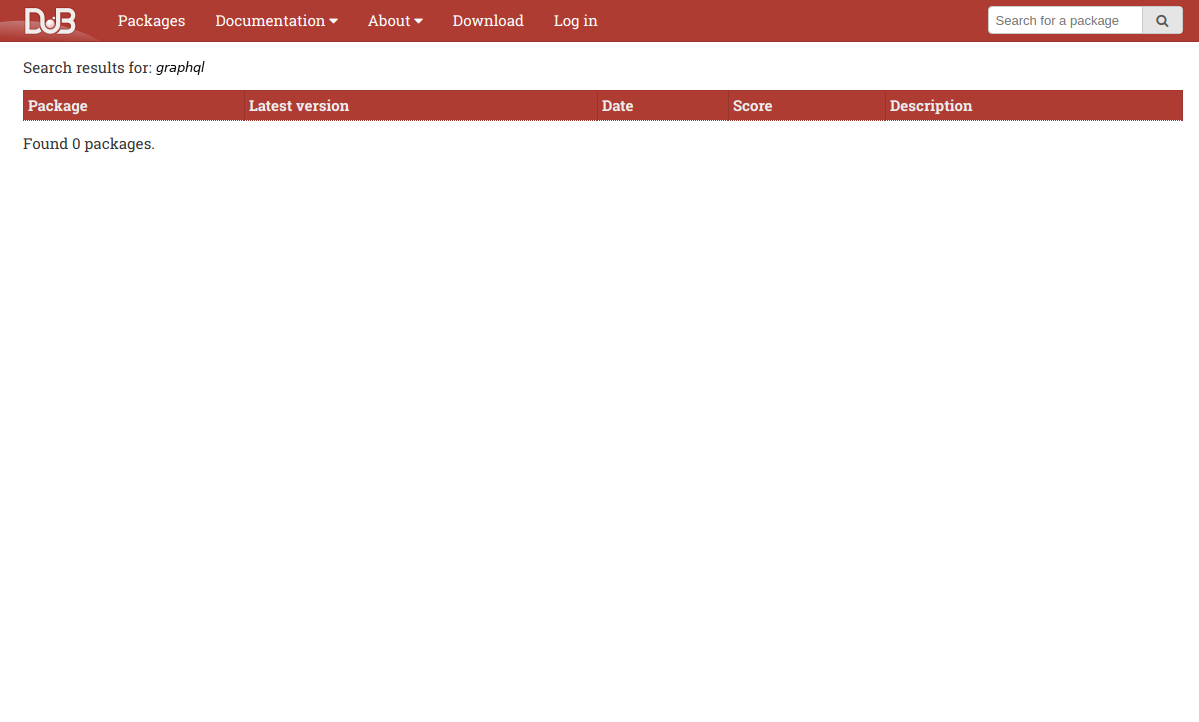
\includegraphics{graphqlsearch.jpg}	
		\end{center}	
	\end{frame}

	\begin{frame}{JUST DO IT}
		\begin{center}
    		\inlineMovie[loop&autostart&start=0&stop=10]{justdoit.mpg}{justdoit-0.png}{height=0.9\textheight}
		\end{center}
	\end{frame}

	\begin{frame}[fragile]{GraphQLD \hfill\cite{graphqld}}
		\begin{columns}[t]
			\begin{column}{0.4\textwidth}
\begin{lstlisting}[language=D,basicstyle=\scriptsize\ttfamily]
import graphqld;

interface Query {
	Employee[] getAllEmployees();
}

class Schema {
	Query queryType;
}
\end{lstlisting}
			\end{column}
	\pause
			\begin{column}{0.6\textwidth}
\begin{lstlisting}[language=D,basicstyle=\scriptsize\ttfamily]
auto graphqld = new GraphQLD!(Schema)();

graphqld.setResolver(
  "queryType", "getAllEmployees",
  delegate(string name, Json parent, 
      Json args, ref Context context) @safe
  {
    Employee[] employees = getAllEmployees();
    Json ret = Json.emptyObject();
    ret["data"] = toGraphqlJson(employees);
    return ret;
  });
\end{lstlisting}
			\end{column}
		\end{columns}
	\end{frame}

	\begin{frame}[fragile]{GraphQLD}
\begin{lstlisting}[language=D,basicstyle=\small\ttfamily]
void graphqlEndpoint(HTTPServerRequest req, 
		HTTPServerResponse res) 
{
	string toParse = extractQuery(req);
	auto p = Parser(Lexer(toParse));

	Document d = p.parseDocument();
	auto fv = new QueryValidator(d);
	auto sv = new SchemaValidator!Schema(d, graphqld.schema);
	fv.accept(d);
	sv.accept(d);

	Context con = buildContext(req);
	Json ret = graphqld.execute(d, extractVariables(req), con);
	res.writeJsonBody(ret);
}
\end{lstlisting}
	\end{frame}

	\begin{frame}[fragile]{GraphQLD}
\begin{lstlisting}[language=D,basicstyle=\small\ttfamily]
graphqld.setResolver("Employee", "info",
  delegate(string name, Json parent, Json args,
      ref Context context)
  {
    const id = parent["infoId"].get!long();
    EmployeeInfo ei = getEmployeeInfo(id);
    Json ret = Json.emptyObject();
    ret["data"] = toGraphqlJson(ei);
    return ret;
  });
\end{lstlisting}
	\end{frame}

	\begin{frame}{GraphQLD}
		\Large
		\begin{itemize}
			\item Mostly feature complete
			\item Some validations are missing
			\item $\approx 17000$ lines
			\item $\approx 9000$ lines are generated by darser
			\item ready for use now
		\end{itemize}	
	\end{frame}

	\section{Homework}
	\begin{frame}[fragile]{Homework}
		\huge
		\begin{center}
			Write a GraphQL backend that uses an excel spreadsheet as a database.
		\end{center}
	\end{frame}

	\section{Conclusion}
	\begin{frame}[fragile]{Conclusion}
		\Large
		\begin{itemize}
			\item Spreadsheets are a terrible programming language. \pause
			\item C++ and Rust are not our main competition.\\[1cm] \pause
			\item We need to learn to use what is there.
			\item Use D to work smart not hard.
			\item Do not write the code, write the code that writes the code.
			\item Look at JS for inspiration.
			\item GraphQL \thumbup{}\\[5mm]
		\end{itemize}
	\end{frame}
	\appendix

	\section{The End}
	\begin{frame}[allowframebreaks]{}
		\printbibliography[heading=none]
	\end{frame}

	\section{Encore}
	\begin{frame}[fragile]{Reappearing UDA Pattern}
\begin{lstlisting}[language=D,basicstyle=\scriptsize\ttfamily]
struct Employee {
	@GQLD(
		Description("The social security number of an employee"),
		Deprecated(IsDeprecated.yes, "To complex")
	)
	SocialSecurityNumber number;
}
\end{lstlisting}
\pause
\begin{lstlisting}[language=D,basicstyle=\scriptsize\ttfamily,firstnumber=9]
enum IsDeprecated {
	undefined,
	no,
	yes
}

struct GQLDData {
	Description desc;
	Deprecated depre;
}
\end{lstlisting}
	\end{frame}

	\begin{frame}[fragile]{Reappearing UDA Pattern}
\begin{lstlisting}[language=D,basicstyle=\footnotesize\ttfamily]
struct GQLDData {
	Description desc;
	Deprecated depre;
}

GQLDData GQLD(Args...)(Args args) {
	GQLDData ret;
	static foreach(mem; __traits(allMembers, GQLDData)) {
		static foreach(arg; args) {
			static if(is(typeof(__traits(getMember, ret, mem)) == 
					typeof(arg))) 
			{
				__traits(getMember, ret, mem) = arg;
			}
		}
	}
	return ret;
}
\end{lstlisting}
	\end{frame}

	\begin{frame}[fragile]{Static Foreach Switch Case}
\begin{lstlisting}[language=D,basicstyle=\footnotesize\ttfamily]
Json ret = Json.emptyObject();
string typename = ...;
l: switch(typename) {
	static foreach(type; collectTypes!(T)) {{
		case typeToTypeName!(type): {
			ret["data"] = typeToJson!(type)();
			break l;
		}
	}}
	default: break;
}
return ret;
\end{lstlisting}
	\end{frame}

	\begin{frame}[fragile]{Collecting all Referenced Types}
\begin{lstlisting}[language=D,basicstyle=\scriptsize\ttfamily]
alias allTypes = collectTypes!Schema;

template collectTypesImpl(Type) {
	import graphql.uda;
	static if(is(Type : GQLDCustomLeaf!F, F)) {
		alias collectTypes Impl= AliasSeq!(Type);
	} else static if(is(Type == interface)) {
		alias RetTypes = AliasSeq!(collectReturnType!(Type,
				__traits(allMembers, Type)));
		alias ArgTypes = AliasSeq!(collectParameterTypes!(Type,
				__traits(allMembers, Type)));
		alias collectTypesImpl = AliasSeq!(Type, RetTypes, 
				ArgTypes, InterfacesTuple!Type);
	....
	} else static if(is(Type == union)) {
		alias collectTypesImpl = AliasSeq!(Type, InheritedClasses!Type);
	} else static if(is(Type : Nullable!F, F)) {
		alias collectTypesImpl = .collectTypesImpl!(F);
	...
\end{lstlisting}
	\end{frame}

	\begin{frame}[fragile]{Compile-Time are long as}
		\Large
		\begin{itemize}
			\item $\approx{} 7000$ lines
			\item $\approx{} 8$ seconds build time
		\end{itemize}
	\end{frame}

	\begin{frame}[fragile]{Overall Legacy Architecture}
		\Large
		\begin{itemize}
			\item Traditional compiler pipeline design is dated
				\pause
			\item We have practically unlimited memory
			\item Recreating the AST, IR, and ASM on every compile is extremely wasteful
			\item Why does code-completion and the compiler different frontends
		\end{itemize}
	\end{frame}

	\begin{frame}{Possible Compiler Re-arch}
		\begin{center}
		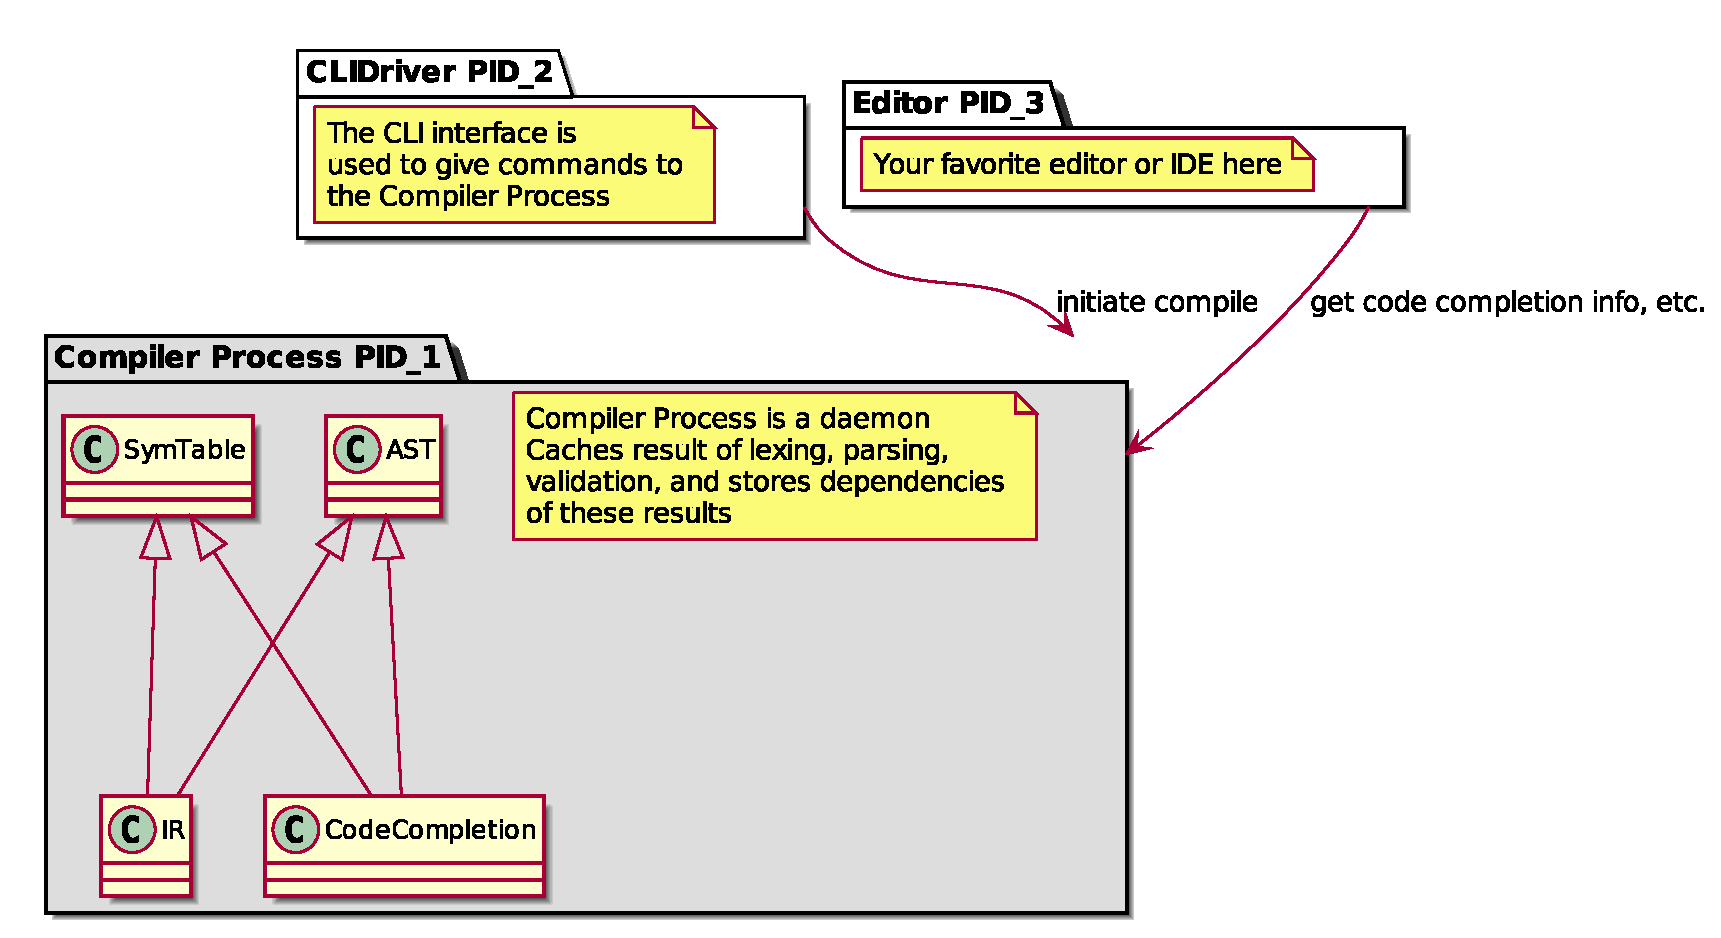
\includegraphics[height=0.9\textheight]{rearch.eps}
		\end{center}
	\end{frame}

	\begin{frame}{Darser \hfill\cite{darser}}
		\begin{itemize}
			\item Darser is a recursive descent parser generator for LL(1) grammars
			\item It also generates the AST and a default Visitor
			\item Not at CT, but as a pre-build step\\[1cm]\pause
			\item It generates ``good'' error messages
			\item Not just a generic Node types, but names that reflect the grammar
			\item Inheriting from the default Visitor is trivial and powerful
			\item Used right now by GraphQLD
		\end{itemize}
	\end{frame}

	\section{I'm out of Slides}
\end{document}
